\chapter{Traditional models}

To estimate a PD model, different types of models varying in complexity are available:

\begin{enumerate}
  \item Statistical Models: This type utilizes historical data for the estimation process. Techniques such as logistic regression, survival analysis and machine learning algorithms are used to predict default events and analyze contributing risk factors.
  \item External Rating Models: Rating agencies develop models that assign credit ratings to borrowers. These models consider various factors, e.g., financial statements and macroeconomic conditions, to evaluate creditworthiness. These types of PD models are only available for a limited portion of borrowers. 
  \item Expert Judgment: In cases where historical data is limited or only a low number of default events is available, expert judgment will become the most relevant. Experienced credit analysts rely on their expertise and industry knowledge to estimate the PD based on qualitative factors, market conditions and client information.
\end{enumerate}

In practice, a substantial portion of the banking sector employs a combination of multiple types of models in their credit risk assessment.

\section{Logit and Probit regression}
Logistic regression is one of the banking industry's most commonly used statistical models. It is practical when the dependent variable is binary. The model estimates the probability of default by fitting a link function to the explanatory variables. Therefore, it transforms the resulting score, which can take any negative or positive value, to the corresponding PD value between 0 and 1. A high model score means a lower probability of default and vice versa. The logistic function or standard normal cumulative distribution function can be used for the link function, resulting in the logit or probit model. An advantage of the logit model is the heavier tails in the logistic distribution, which would put higher weights on extreme events. \cite[pp.~40-42]{Witzany:2017}

\begin{figure}[H]
\begin{minipage}{.5\textwidth}
	\begin{equation}
	f(x) = \frac{1}{1 + e^{-x}}
	\end{equation}
\end{minipage}%
\begin{minipage}{.5\textwidth}
	\centering
	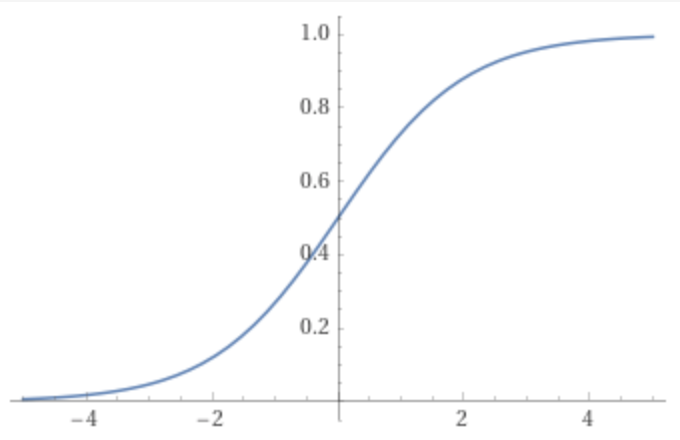
\includegraphics[width=.5\textwidth]{./TM__logistic_func.png}
\end{minipage}
    \caption{Logistic Function}
    \label{fig:tm_logfunc}
\end{figure}

\section{Other Models}

\subsection{Linear regression}
During the linear regression, the algorithm estimates a linear relationship between the default variable, which assumes either the value 0 (non-default) or 1 (default), and explanatory variables, which can be continuous and categorical independent variables, such as income, employment duration and profession. Unfortunately, due to the binary dependent variable, the residuals are heteroscedastic; therefore, the coefficients' estimation is inefficient. Additionally, the model may output non-logical results, like negative values or a PD over 100\%. \cite[pp.~39-40]{Witzany:2017}

\subsection{External Ratings}
Scorings of corporate clients are usually performed mainly by a credit analyst and only partly automated due to the low number of default events and the type of information available. External ratings may be used if the financial institution needs more resources to develop and maintain internal models. The most known rating agencies are Standard \& Poor, Moody's and Fitch. They provide ratings for a wide range of corporations since most companies request a rating before a sale or registration of a debt issue. An analyst will use their financial statements of the last few years and additional information to derive a rating, which is then discussed in a rating committee. Afterward, the corporation is informed about its rating and the corresponding factors and given the opportunity to respond; finally, the ratings will be published. A disadvantage of external ratings observed in the past is the conflict of interest since the company mainly pays the ratings. It is suspected that good ratings were related to high fees, visible during the financial crisis, where many structured bonds with high scorings deteriorated unexpectedly. \cite[pp.~34-36]{Witzany:2017}

\subsection{Shadow Rating}
The Shadow Rating approach aims to estimate a model that produces similar PDs as ratings determined by external rating agencies. For this process, possible input factors, for example, macroeconomic factors and financial statements, need to be defined. The model's output serves as a valuable tool for credit analysts in making the final decisions. \cite[pp.~67]{Witzany:2017}